\section{Matrix-based multiple-source CFPQ algorithm}
\label{sec:multiple-source-algo}
 In this section we introduce two versions of multiple-source matrix-based CFPQ algorithm. This algorithm is a modification of Azimov's matrix-based algorithm for CFPQ and its idea is that we cut off those vertices from which we are not interested in paths.
 
 Let \mbox{$D = (V, E)$} be the input graph, \mbox{$G = (N, \Sigma, P)$} be the input context-free grammar and $Src$ be the input set of vertices. For the multiple-source context-free path query evaluation for every $A \in Src$ we need to find all context-free relations $R_A$, i.e. all node pairs \mbox{$(n,m)$} such that \mbox{$\exists n \pi m~(l(\pi) \in L(G_A))$}.
\begin{algorithm}
\begin{algorithmic}[1]
\caption{Multiple-source context-free path querying algorithm}
\label{alg:algo1}
\Function{MultiSrcCFPQ}{$D=(V,E), G=(N,\Sigma,P,S), Src$}
    \State{$T \gets \{T^A \mid  A \in N, T^A \gets \emptyset\}$}
    \Comment{Matrix in which every element is $\emptyset$}
    
    \State{$TSrc \gets \{TSrc^A \mid  A \in N \setminus S, TSrc^A \gets \emptyset\}$}
    \Comment{Matrix for input vertices in which every element is $\emptyset$}

    \ForAll{$ v \in Src$} \Comment{Input matrix initialization}
        \State{$TSrc^S_{v,v} \gets true$} 
    \EndFor

    \ForAll{$A \to x \in P$} \Comment{Simple rules initialization}
        \ForAll{$(v, x, to) \in E$}
            \State{$T^A_{v,to} \gets true$}
        \EndFor
    \EndFor

    \While{$T\ or\ TSrc\ is\ changing$} \Comment{Algorithm's body}
        \ForAll{$A \to B C \in P$}
            \State{$M \gets TSrc^A*T^B$}
            \State{$T^A \gets T^A + M*T^C$}
            \State{$TSrc^B \gets TSrc^B + TSrc^A$}
            \State{$TSrc^C \gets TSrc^C + $ \Call{getDst}{M}}
        \EndFor
    \EndWhile
    \State \Return T
\EndFunction

\\

\Function{getDst}{M}
    \State{$A \gets \emptyset$}
    \ForAll{$(v,to) \in V^2 \mid M_{v,to} = true$}
        \State{$A_{to,to} \gets true$}
    \EndFor
    \State \Return A
\EndFunction
\end{algorithmic}
\end{algorithm}
In order to solve the single-source and multiple-source CFPQ problem Azimov's algorithm was modified: operations of Boolean matrix multiplication $T_A = T_A + T_B \cdot T_C$ for each $A \rightarrow BC \in R$ represented in line \textbf{8} of Algorithm~\ref{alg:algo0} was supplemented with one more matrix multiplication $T_A = T_A + (TSrc^A \cdot T_B) \cdot T_C$ for each $A \rightarrow BC \in R$ which saves only vertices we are interested in, where $TSrc^A$ --- matrix of vertices to calculate the paths from. It is represented in lines \textbf{11-13} of the Algorithm~\ref{alg:algo1}. Also, after every iteration of while loop this is nessesary to update the set of vertices paths from which we need to calculate. To do this, the function \textbf{getDst}, represented in lines \textbf{17-21}, is called at line \textbf{14}. Thus, the modified algorithm does not calculate the paths from all vertices in case of query to calculate the paths small set of vertices.

We proposed the variant of the algorithm that can calculate the paths from a certain set of vertices, however there are such scenarios when queries are partially or completely repeated. In such cases it would be useful to add data caching to improve the performance. The problem is that every time we want to find all paths from the certain set of vertices, the Algorithm~\ref{alg:algo1} calculates everything from scratch. Since recalculating might take the significant amount of time, we modified multiple-source CFPQ algorithm to specify it for such scenarios. This version stores all the vertices the paths from which have already been calculated in cash $index$, which is used to filter such vertices in line \textbf{3} of Algorithm~\ref{alg:algo2}. Thus, modified algorithm calculates paths from the particular vertex only once.
\begin{algorithm}
\begin{algorithmic}[1]
\caption{Optimized multiple-source context-free path querying algorithm}
\label{alg:algo2}
\Function{MultiSrcCFPQSmart}{$index=(D, G, T, TSrc), Src$}
    \State{$TNewSrc \gets \{TNewSrc^A \mid  A \in N \setminus S, TNewSrc^A \gets \emptyset\}$}

    \ForAll{$v \in Src \mid index.TSrc_{v,v} = false$}
        \State{$TNewSrc^S_{v,v} \gets true$}
    \EndFor

    \While{$index.T\ or\ TNewSrc\ is\ changing$}
        \ForAll{$A \to B C \in P$}
            \State{$M \gets TNewSrc^A*index.T^B$}
            \State{$index.T^A \gets index.T^A + M*index.T^C$}

            \State{$TNewSrc^B \gets TNewSrc^B + TNewSrc^A \setminus index.TSrc^B$}
            \State{$TNewSrc^C \gets TNewSrc^C + $ \Call{getDst}{M}} $\setminus$ $index.TSrc^C$
        \EndFor
    \EndWhile
\EndFunction


\end{algorithmic}
\end{algorithm}

\subsection{Implementation Details}

 All of the above versions have been implemented$\footnote{GitHub repository with implemented algorithms: \url{https://github.com/JetBrains-Research/CFPQ_PyAlgo}, last accessed 28.08.2020}$ using GraphBLAS framework that allows you to represent graphs as matrices and work with them in terms of linear algebra. For convenience, all the code is written in Python using pygraphblas\footnote{GitHub repository of PyGraphBLAS library: \url{https://github.com/michelp/pygraphblas}}, which is Python wrapper around GraphBLAS API and based on SuiteSparse:GraphBLAS\footnote{GitHub repository of SuiteSparse:GraphBLAS library: \url{https://github.com/DrTimothyAldenDavis/SuiteSparse}}~\cite{10.1145/3322125} --- the full implementation of GraphBLAS standard. This library is specialized for working with sparse matrices, which most often appear in real graphs. Also, it should be noted that, despite the fact that the function \textbf{getDst} does not seem to be expressed in terms of linear algebra, the implementation used the function \textbf{reduce\_vector} from pygraphblas that reduces matrix to a vector, with which further work takes place.

\subsection{Algorithm Evaluation}

We evaluate both described version of multiple-source algorithm on real-world graphs.
For evaluation, we use a PC with Ubuntu 20.04 installed.
It has Intel core i7-4790 CPU, 3.60GHz, and DDR3 32Gb RAM.
As far as we evaluate only algorithm execution time, we store each graph fully in RAM as its adjacency matrix in sparse format.
Note, that graph loading time is not included in the result time of evaluation. 

For evaluation we use graphs and queries from CFPQ\_Data dataset\footnote{CFPQ\_Data is a dataset for CFPQ evaluation which contains both synthetic and real-world data and queries \url{https://github.com/JetBrains-Research/CFPQ\_Data}, last accessed 28.08.2020.}
Detailed information on graphs which we select for evaluation is provided in table~\ref{tbl:graphs_for_cfpq}.
We use classical same-generation queries $G_1$~(eq.~\ref{eqn:g_1}) and $G_2$~(eq.~\ref{eqn:g_2}) which are used in other works for CFPQ evaluation. 
Also we use $Geo$~(eq.~\ref{eqn:geo}) query which was provided by J. Kuijpers et. al~\cite{Kuijpers:2019:ESC:3335783.3335791} for \textit{geospecies} RDF.
Note that in queries we use $\overline{x}$ notation to denote inverse of $x$ relation and respective edge.
\begin{align}
\begin{split}
\label{eqn:g_1}
S \to & \overline{\textit{subClassOf}} \ \ S \ \textit{subClasOf} \mid \overline{\textit{type}} \ \ S \ \textit{type}\\   & \mid \overline{\textit{subClassOf}} \ \ \textit{subClasOf} \mid \overline{\textit{type}} \ \textit{type}
\end{split}
\end{align}
\begin{align}
\label{eqn:g_2}
S \to \overline{\textit{subClassOf}} \ \ S \ \textit{subClasOf} \mid \textit{subClassOf}
\end{align}
\begin{align}
\begin{split}
\label{eqn:geo}
S \to & \textit{broaderTransitive} \ \  S \ \overline{\textit{broaderTransitive}} \\
      & \mid \textit{broaderTransitive} \ \  \overline{\textit{broaderTransitive}}
\end{split}
\end{align}

{\setlength{\tabcolsep}{0.2em}
\begin{table}
{
\caption{Graphs for CFPQ evaluation}
\label{tbl:graphs_for_cfpq}
\small
\rowcolors{2}{black!2}{black!10}
\begin{tabular}{|l|c|c|c|c|c|}
\hline
Graph          & \#V       & \#E        & \#subCalssOf & \#type &\#broaderTransitive\\
\hline
\hline 
core           &           &            &              &        &        ---        \\
eclass\_514en  &           &            &              &        &        ---        \\
enzyme         &           &            &              &        &        ---        \\
geospecies     &           &            &              &        &                   \\
go             &           &            &              &        &        ---        \\
go-hierarchy   &           &            &              &        &        ---        \\
pathways       &           &            &              &        &        ---        \\
taxonomy       &           &            &              &        &        ---        \\
\hline
\end{tabular}
}
\end{table}
}


Our main goal is to compare behavior of two proposed versions of the algorithm.
To do it we measure query execution time for both versions for different sizes of star vertex set. 
Namely, for each graph we split all vertices into disjoint subsets of fixed size.
After that, for each subset we evaluate queries using the given subset as a set of start vertices. 

Results of evaluation is presented in figures !!!!.
\begin{figure}
     \begin{subfigure}[b]{0.24\textwidth}
         \centering
         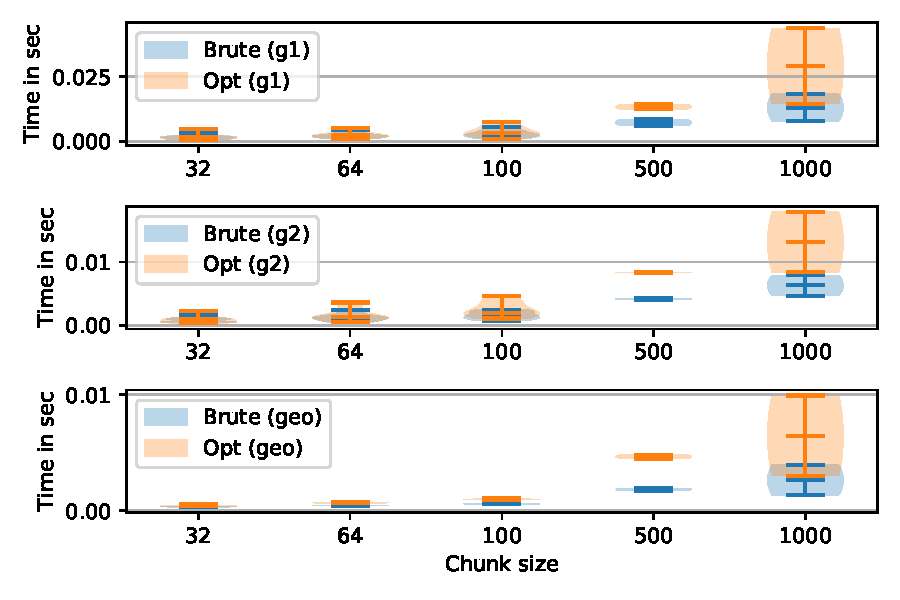
\includegraphics[width=\textwidth]{data/raw/core.pdf}
         \caption{$y=x$}
         \label{fig:y equals x}
     \end{subfigure}
     ~\begin{subfigure}[b]{0.24\textwidth}
         \centering
         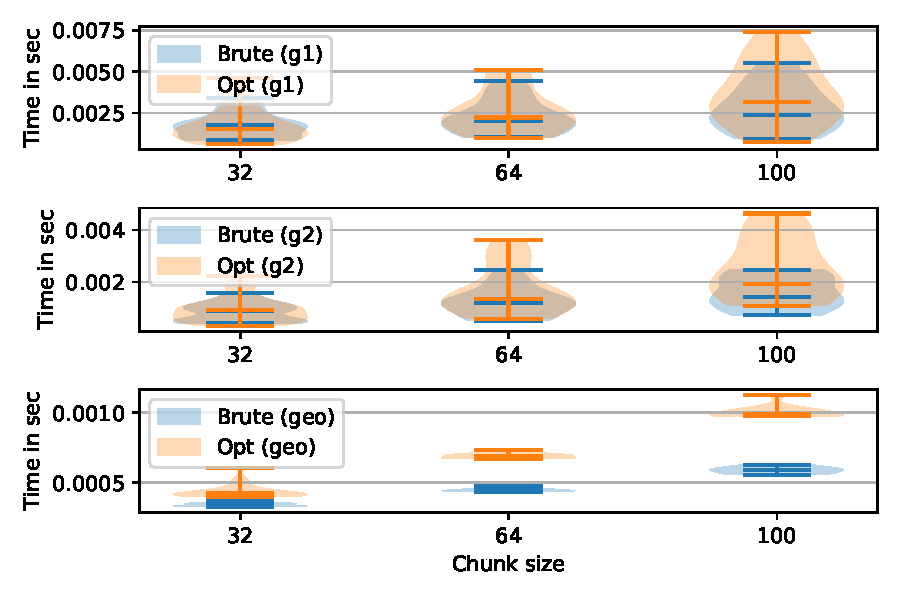
\includegraphics[width=\textwidth]{data/raw/core_3.pdf}
         \caption{$y=x$}
         \label{fig:y equals x}
     \end{subfigure}\\
   \caption{Single path extraction}
\end{figure}


\begin{figure}[h]
\centering
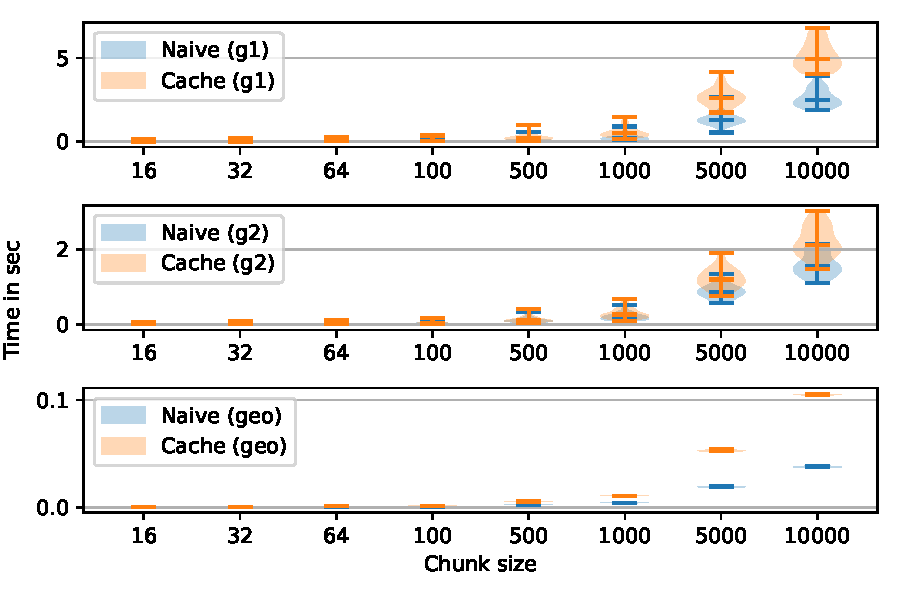
\includegraphics[width=0.5\textwidth]{data/raw/go.pdf}
\caption{Example of a parametric plot ($\sin (x), \cos(x), x$)}
\end{figure}

\begin{figure}[h]
\centering
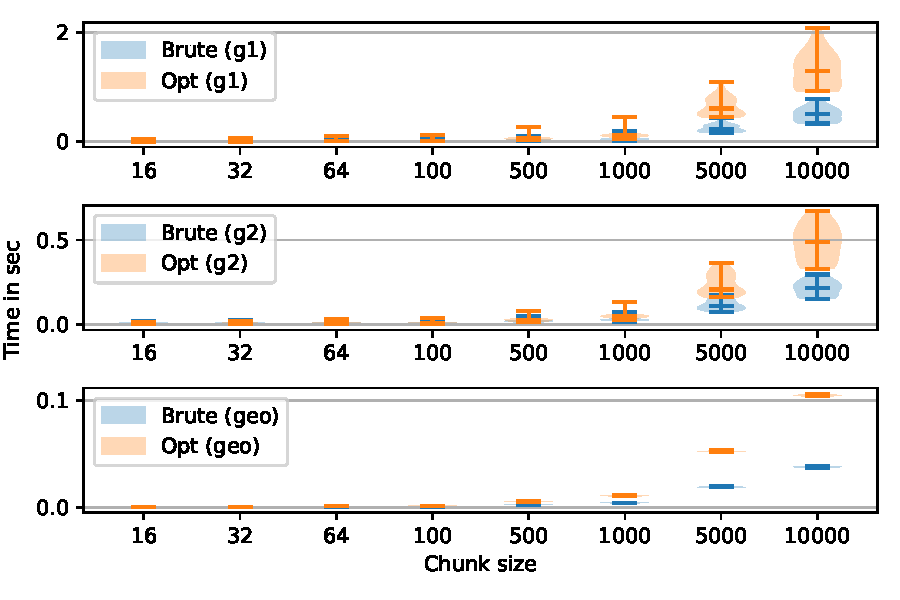
\includegraphics[width=0.5\textwidth]{data/raw/eclass_514en.pdf}
\caption{Example of a parametric plot ($\sin (x), \cos(x), x$)}
\end{figure}

\begin{figure}[h]
\centering
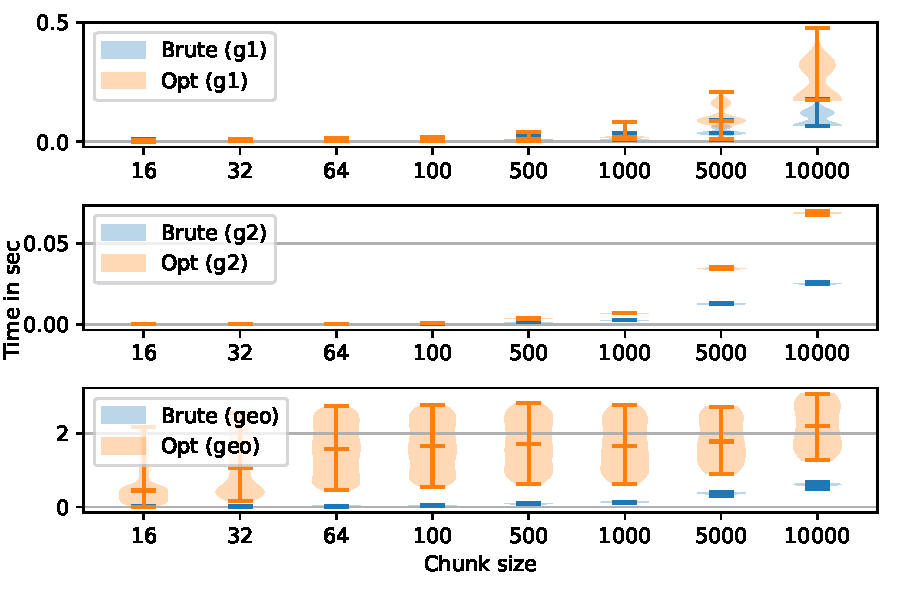
\includegraphics[width=0.5\textwidth]{data/raw/geospecies.pdf}
\caption{Example of a parametric plot ($\sin (x), \cos(x), x$)}
\end{figure}

\begin{figure}[h]
\centering
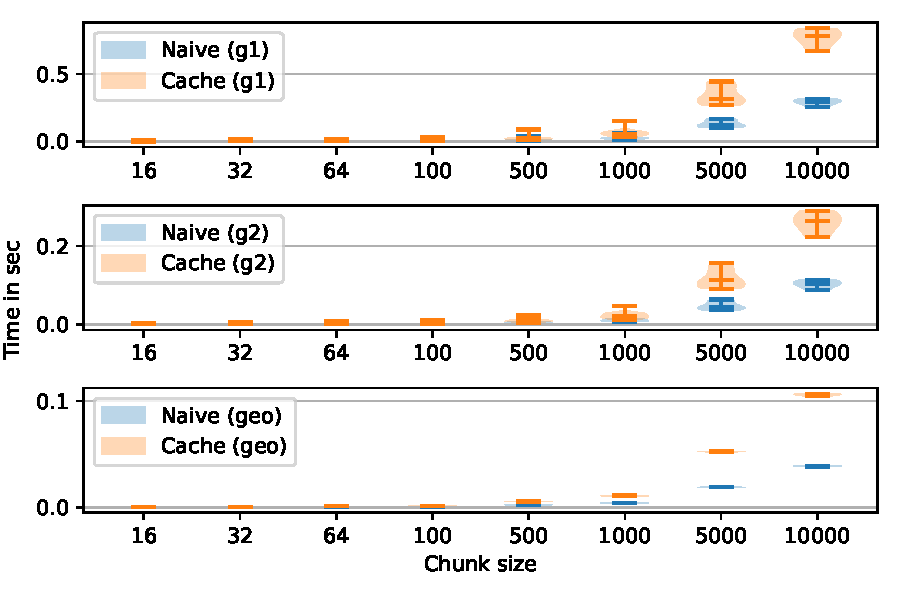
\includegraphics[width=0.5\textwidth]{data/raw/enzyme.pdf}
\caption{Example of a parametric plot ($\sin (x), \cos(x), x$)}
\end{figure}

\begin{figure}[h]
\centering
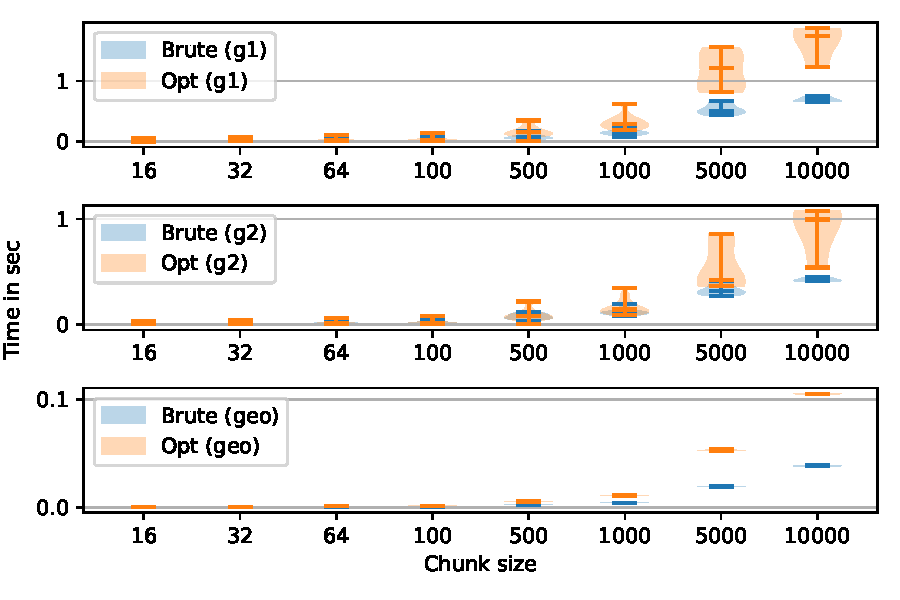
\includegraphics[width=0.5\textwidth]{data/raw/gohierarchy.pdf}
\caption{Example of a parametric plot ($\sin (x), \cos(x), x$)}
\end{figure}


\begin{figure}[h]
\centering
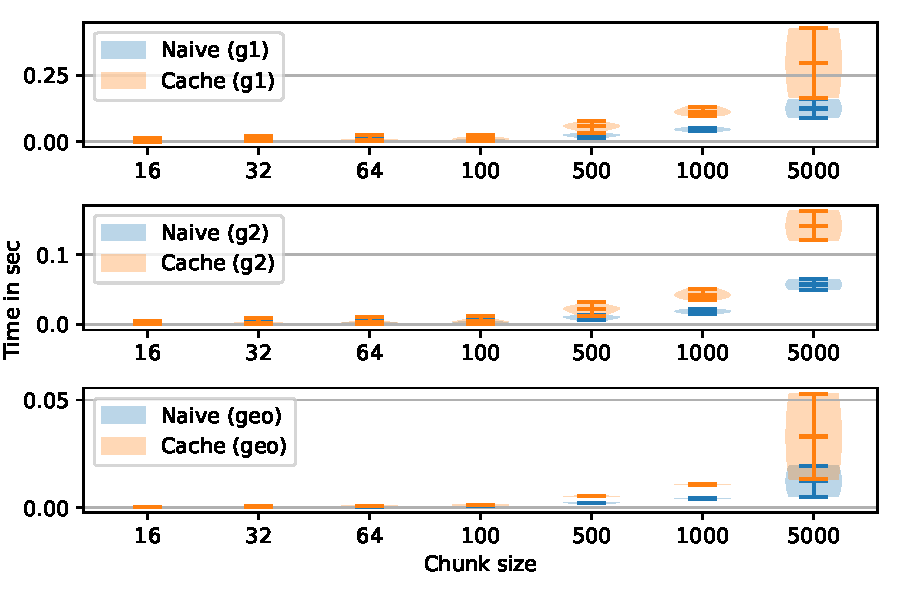
\includegraphics[width=0.5\textwidth]{data/raw/pathways.pdf}
\caption{Example of a parametric plot ($\sin (x), \cos(x), x$)}
\end{figure}


We can see, that ....
As a result, we select !!! to integrate into RedisGraph!!!